% Deep Generative Models: A Visual Overview (2025)
% Author: Your Name
% Compile: pdflatex (twice) or latexmk
\documentclass[aspectratio=169]{beamer}

% ==== Theme & basic look ====
\usetheme{Madrid}
\usecolortheme{seahorse}
\setbeamertemplate{navigation symbols}{}
\setbeamertemplate{footline}[frame number]

% ==== Packages ====
\usepackage[T1]{fontenc}
\usepackage[utf8]{inputenc}
\usepackage{amsmath, amssymb}
\usepackage{booktabs}
\usepackage{graphicx}
\usepackage{xcolor}
\usepackage{adjustbox}
\usepackage{tikz}
\usetikzlibrary{arrows.meta,positioning,calc,fit,shadows}
% scale all TikZ a bit smaller to avoid overflow
\tikzset{every picture/.style={scale=0.9, transform shape}}

% ==== Colors & helpers ====
\definecolor{myblue}{RGB}{13,71,161}
\definecolor{mygreen}{RGB}{27,94,32}
\definecolor{myorange}{RGB}{230,81,0}
\definecolor{myviolet}{RGB}{94,53,177}
\definecolor{mygray}{RGB}{97,97,97}

\newcommand{\placeholderfig}{% 
  \begin{center}
    \begin{adjustbox}{max size={\linewidth}{.65\textheight}}
      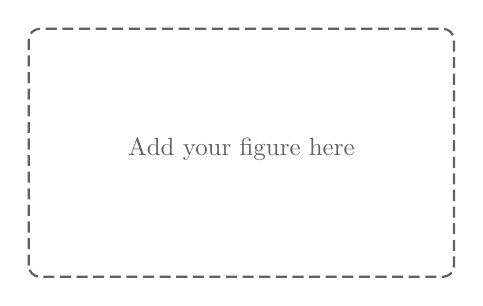
\begin{tikzpicture}[x=1cm,y=1cm]
        \draw[rounded corners, dash pattern=on 4pt off 2pt, line width=0.8pt, mygray] (0,0) rectangle (6,3.5);
        \node[mygray] at (3,1.8) {Add your figure here};
      \end{tikzpicture}%
    \end{adjustbox}
  \end{center}%
}

% Small checkmark and cross
\newcommand{\cmark}{\textcolor{mygreen}{\ensuremath{\checkmark}}}
\newcommand{\xmark}{\textcolor{red}{\ensuremath{\times}}}

% Title page details:   
\title[Large Foundation models]{Large Foundation Models: Mathematics, Algorithms, and Applications
}  
\author{Pipi Hu}  
\institute[BIMSA]{Beijing Institute of Mathematical Sciences and Applications}  
\date{\today}  

\pgfdeclareimage[width=2cm]{logo}{figs/logo.png}
\logo{\pgfuseimage{logo}{\vspace{-6pt}}}

\begin{document}

% ---------------- Title Page ----------------
\begin{frame}
  \titlepage
\end{frame}

% ---- Learning Objectives ----
\begin{frame}{Learning Objectives}
\small
By the end of this course you will be able to:
\begin{itemize}
  \item Explain what it means to learn a data distribution $p_\theta(\mathbf{x})$ or a conditional $p_\theta(\mathbf{x}\mid\mathbf{c})$.
  \item Compare the five major families: Autoregressive, VAE, GAN, Normalizing Flows, Diffusion/Flow Matching.
  \item Relate their training objectives to a unifying divergence/likelihood view.
  \item Distinguish training vs. sampling costs and typical latency/quality trade-offs.
  \item Choose an appropriate model family for a task, and see how world models connect to these tools.
  \item Understanding how the reinforcement learning works.
  \item Construct your own Models.
\end{itemize}
\end{frame}

% ---------------- Agenda ----------------
\begin{frame}{Agenda}
  \tableofcontents
\end{frame}

% ---- New Prologue slide inserted here ----
\begin{frame}{Preliminary: The Bitter Lesson (Sutton)}
\small
\textbf{Thesis.} Hand-crafted domain knowledge scales poorly; progress comes from \textit{general-purpose} methods that learn directly from data with lots of compute. Design \textbf{mathematical learning algorithms} so models \textit{acquire} the distribution, rather than hard-coding it.

\vspace{0.35em}
\textbf{Implications for deep generative modeling}
\begin{itemize}
  \item Prefer scalable objectives: maximize $\log p_\theta(\mathbf{x})$ or minimize a divergence $D( p_{\text{data}} \Vert p_\theta )$; use variational bounds/score objectives.
  \item Use generic, data-driven representations (Transformers, CNNs, U-Nets, invertible nets) \textit{+} self-supervision.
  \item Scale data/compute; reduce bespoke heuristics and narrow domain rules (\xmark \; brittle, hard to scale).
\end{itemize}

\vspace{0.35em}
\begin{center}
\begin{adjustbox}{max size={\linewidth}{.45\textheight}}
  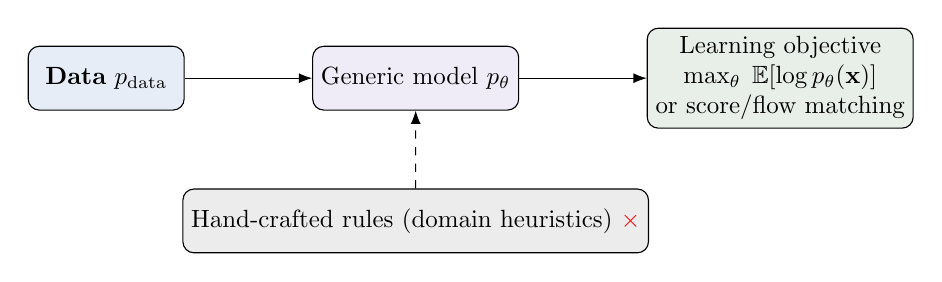
\begin{tikzpicture}[node distance=1.4cm]
    \tikzstyle{box}=[draw, rounded corners, minimum width=2.2cm, minimum height=0.9cm, align=center]
    \node[box, fill=myblue!10] (data) {\textbf{Data} $p_{\text{data}}$};
    \node[box, right=1.8cm of data, fill=myviolet!10] (model) {Generic model $p_\theta$};
    \node[box, right=1.8cm of model, fill=mygreen!10] (learn) {Learning objective\\$\max_\theta \; \mathbb{E}[\log p_\theta(\mathbf{x})]$\\ or score/flow matching};
    \draw[-{Latex}] (data) -- (model);
    \draw[-{Latex}] (model) -- (learn);
    \node[below=1.1cm of model, box, fill=gray!15] (rules) {Hand-crafted rules\ (domain heuristics) \xmark};
    \draw[-{Latex}, dashed] (rules.north) -- (model.south);
  \end{tikzpicture}
\end{adjustbox}
\end{center}

\end{frame}

% ================= Section ==================
\section{What is Generative Modeling?}

\begin{frame}{Definition and Why It Matters}
Generative models learn a distribution $p(\mathbf{x})$ (or $p(\mathbf{x}\,|\,\mathbf{c})$) over complex data (images, text, audio, video, 3D, proteins), enabling:
\begin{itemize}
  \item \textbf{Synthesis} (sample new $\mathbf{x}$), \textbf{imputation}, \textbf{editing}, \textbf{control}, \textbf{compression}.
  \item As world-model primitives for \textbf{simulation}, \textbf{planning}, \textbf{data augmentation}.
\end{itemize}
\vspace{0.5em}
Two big families of objectives:
\begin{enumerate}
  \item \textbf{Likelihood/variational} training (maximize $\log p_\theta(\mathbf{x})$ or its bound).
  \item \textbf{Adversarial/implicit} training (match data distribution without tractable likelihood).
\end{enumerate}
\end{frame}

% ---- Notation & Setup ----
\begin{frame}{Notation \& Setup}
\small
\begin{itemize}
  \item Data: $\mathcal{D}=\{\mathbf{x}^{(i)},\mathbf{c}^{(i)}\}_{i=1}^N$, variables may be continuous \emph{or} discrete.
  \item Parameters: $\theta$; latent variables (when present): $\mathbf{z}$; tokenizer/codebook: $\mathcal{Z}$.
  \item Objectives: maximize $\log p_\theta$, minimize divergence $D( p_{\text{data}} \Vert p_\theta )$, or match a transport/flow.
  \item Inference artifacts: decoders, samplers, inverse maps; report both \textit{train cost} and \textit{sample latency}.
\end{itemize}
\end{frame}

% ---- Unifying View ----
\begin{frame}{A Unifying Objective View}
\begin{table}
\centering
\begin{tabular}{@{}l l@{}}
\toprule
Family & Canonical objective (sketch) \\
\midrule
Autoregressive & $\max_\theta \sum_i \log p_\theta(x_i \mid x_{<i})$ (exact NLL) \\
VAE & ELBO: $\mathbb{E}_{q_\phi}[\log p_\theta(\mathbf{x}\mid\mathbf{z})]-\mathrm{KL}[q_\phi(\mathbf{z}\mid\mathbf{x})\Vert p(\mathbf{z})]$ \\
GAN & $\min_G \max_D$ JS/$f$-divergence matching (implicit likelihood) \\
Flows & $\log p_\theta(\mathbf{x})=\log p(\mathbf{z})+\log \lvert \det \partial f/\partial \mathbf{x} \rvert$ \\
Diffusion/Score & Denoising/score matching; flow/consistency matching \\
\bottomrule
\end{tabular}
\end{table}
\vspace{2em}
\textbf{Takeaway:} same destination (match $p_\theta$ to data), different parameterizations and training signals.
\end{frame}

% ---- Training vs Sampling ----
\begin{frame}{Training vs. Sampling Pipelines}
\small
\begin{itemize}
  \item \textbf{Autoregressive:} train once (teacher forcing); sample sequentially (slow, exact likelihood).
  \item \textbf{Diffusion:} train denoiser/score; sample iteratively (few-step via distillation/consistency/flow matching).
  \item \textbf{Flows:} train invertible map; sample in one inverse pass (exact likelihood).
  \item \textbf{VAE:} train encoder/decoder; sample via prior $p(\mathbf{z})$ and decode.
  \item \textbf{GAN:} min-max training; fast single-pass sampling.
\end{itemize}
\centering
\begin{adjustbox}{max size={\linewidth}{.45\textheight}}
  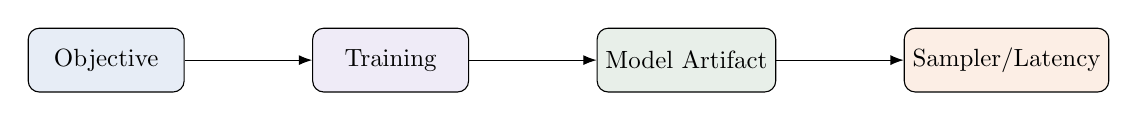
\begin{tikzpicture}[node distance=1.3cm]
    \tikzstyle{b}=[draw, rounded corners, minimum width=2.2cm, minimum height=0.9cm, align=center]
    \node[b, fill=myblue!10] (obj) {Objective};
    \node[b, right=1.8cm of obj, fill=myviolet!10] (train) {Training};
    \node[b, right=1.8cm of train, fill=mygreen!10] (artifact) {Model Artifact};
    \node[b, right=1.8cm of artifact, fill=myorange!10] (sample) {Sampler/Latency};
    \draw[-{Latex}] (obj) -- (train);
    \draw[-{Latex}] (train) -- (artifact);
    \draw[-{Latex}] (artifact) -- (sample);
  \end{tikzpicture}
\end{adjustbox}
\end{frame}

\begin{frame}{A Landscape View}
\centering
\begin{adjustbox}{max size={\linewidth}{.70\textheight}}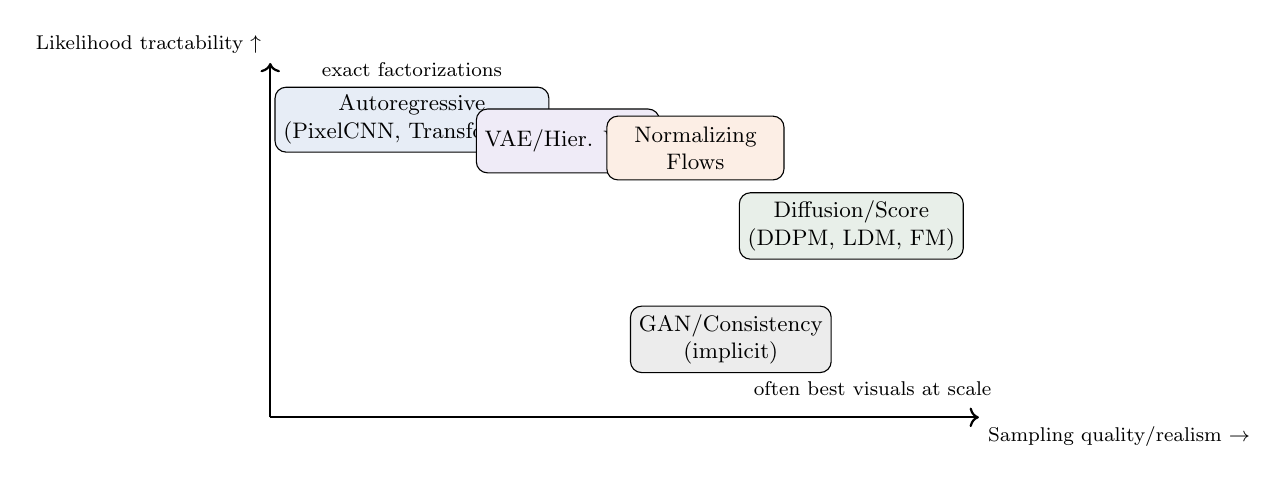
\begin{tikzpicture}[node distance=1.0cm, every node/.style={font=\small}]
  % Axes
  \draw[->,thick] (0,0) -- (10,0) node[below right]{\footnotesize Sampling quality/realism $\rightarrow$};
  \draw[->,thick] (0,0) -- (0,5) node[above left]{\footnotesize Likelihood tractability $\uparrow$};

  % Buckets
  \node[draw, rounded corners, fill=myblue!10, align=center, minimum width=2.5cm, minimum height=0.9cm] (AR) at (2.0,4.2) {Autoregressive\\(PixelCNN, Transformer)};
  \node[draw, rounded corners, fill=myviolet!10, align=center, minimum width=2.5cm, minimum height=0.9cm] (VAE) at (4.2,3.9) {VAE/Hier. VAE};
  \node[draw, rounded corners, fill=myorange!10, align=center, minimum width=2.5cm, minimum height=0.9cm] (FLOW) at (6.0,3.8) {Normalizing\\Flows};
  \node[draw, rounded corners, fill=mygreen!10, align=center, minimum width=2.5cm, minimum height=0.9cm] (DIFF) at (8.2,2.7) {Diffusion/Score\\(DDPM, LDM, FM)};
  \node[draw, rounded corners, fill=gray!15, align=center, minimum width=2.5cm, minimum height=0.9cm] (GAN) at (6.5,1.1) {GAN/Consistency\\(implicit)};

  % Labels
  \node at (2.0,4.9) {\footnotesize exact factorizations};
  \node at (8.5,0.4) {\footnotesize often best visuals at scale};
\end{tikzpicture}\end{adjustbox}
\end{frame}

% ================= Section ==================
\section{Autoregressive (AR) Models}

\begin{frame}{Auto regressive modeling}
\textbf{Factorization:}
\begin{equation*}
  p(\mathbf{x}) = \prod_{i=1}^{D} p\big(x_i\mid x_{<i}\big), \quad \text{with an order over dimensions/tokens.}
\end{equation*}
\vspace{-0.3em}
\begin{itemize}
  \item Image: raster-scan pixels (PixelRNN/CNN); Text/Code: token-by-token (Transformers);
  \item Audio: next-sample prediction (WaveNet); Vision tokens via VQ-VAE + Transformer.
\end{itemize}
\vspace{0.5em}
\textbf{Training:} teacher forcing, \textbf{objective} $\sum_i \log p_\theta(x_i\mid x_{<i})$.
\end{frame}

\begin{frame}{Tiny Graphical Intuition}
\centering
\begin{adjustbox}{max size={\linewidth}{.70\textheight}}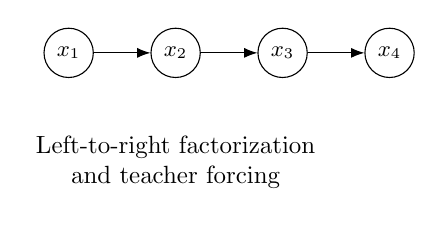
\begin{tikzpicture}[node distance=0.8cm]
  \tikzstyle{var}=[circle, draw, minimum size=6mm, font=\small]
  \node[var] (x1) {$x_1$};
  \node[var, right=of x1] (x2) {$x_2$};
  \node[var, right=of x2] (x3) {$x_3$};
  \node[var, right=of x3] (x4) {$x_4$};
  \draw[-{Latex}] (x1) -- (x2);
  \draw[-{Latex}] (x2) -- (x3);
  \draw[-{Latex}] (x3) -- (x4);
  \node[below=0.7cm of x2, align=center] {Left-to-right factorization\\and teacher forcing};
\end{tikzpicture}\end{adjustbox}
\vspace{0.7em}
\begin{itemize}
  \item \textbf{Pros:} exact likelihood, strong modeling of local dependencies, state-of-the-art in text/code.
  \item \textbf{Cons:} slow sampling (sequential), exposure bias; 2D structure needs careful ordering.
\end{itemize}
\end{frame}

\begin{frame}{Masked vs. AR, and Speed-ups}
\begin{itemize}
  \item \textbf{Masked language modeling (MLM)} learns to fill blanks; not strictly AR but can be combined (e.g., \emph{prefix-decoding}, parallel decoding with iterative refinement).
  \item \textbf{Parallel/Speculative decoding, KV caching, medusa heads} reduce latency.
  \item \textbf{Discretization pipelines:} VQ-VAE/tokenizers + AR over tokens for images/audio/video.
\end{itemize}
\end{frame}

% ================= Section ==================
\section{Variational Autoencoders (VAE)}

\begin{frame}{VAE: Idea and Objective}
\centering
\begin{adjustbox}{max size={\linewidth}{.50\textheight}}
  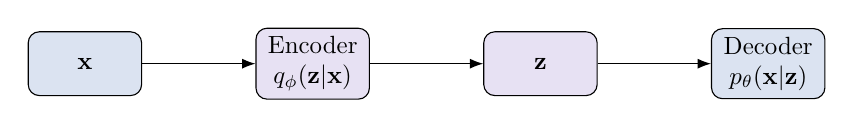
\begin{tikzpicture}[node distance=1.0cm]
    \tikzstyle{box}=[draw, rounded corners, minimum width=1.6cm, minimum height=0.9cm, align=center]
    \node[box, fill=myblue!15] (x) {$\mathbf{x}$};
    \node[box, right=1.6cm of x, fill=myviolet!15] (enc) {Encoder\\$q_\phi(\mathbf{z}|\mathbf{x})$};
    \node[box, right=1.6cm of enc, fill=myviolet!15] (z) {$\mathbf{z}$};
    \node[box, right=1.6cm of z, fill=myblue!15] (dec) {Decoder\\$p_\theta(\mathbf{x}|\mathbf{z})$};
    \draw[-{Latex}] (x) -- (enc);
    \draw[-{Latex}] (enc) -- (z);
    \draw[-{Latex}] (z) -- (dec);
  \end{tikzpicture}
\end{adjustbox}

\vspace{0.6em}
\begin{columns}[T]
  \begin{column}{0.98\linewidth}
    \textbf{Encoder--Decoder with latent $\mathbf{z}$}
    \begin{equation*}
      \log p_\theta(\mathbf{x}) \ge \underbrace{\mathbb{E}_{q_\phi(\mathbf{z}|\mathbf{x})}[\log p_\theta(\mathbf{x}|\mathbf{z})]}_{\text{reconstruction}} - \underbrace{\mathrm{KL}\big(q_\phi(\mathbf{z}|\mathbf{x})\,\Vert\,p(\mathbf{z})\big)}_{\text{regularization}}
    \end{equation*}
  \end{column}
\end{columns}
\vspace{0.3em}
\textbf{Notes:} hierarchical VAEs, \emph{\!\!$\beta$\!-VAE}, vector-quantized VAEs (VQ-VAE), diffusion/AR decoders.
\end{frame}

% ================= Section ==================
\section{GANs (Implicit Models)}

\begin{frame}{GANs: Adversarial Training}
\begin{equation*}
  \min_G \max_D \; \mathbb{E}_{\mathbf{x}\sim p_{\text{data}}}[\log D(\mathbf{x})] + \mathbb{E}_{\mathbf{z}\sim p(\mathbf{z})}[\log (1 - D(G(\mathbf{z})))]
\end{equation*}
\begin{itemize}
  \item \textbf{Pros:} often sharp, realistic samples; once trained, fast sampling.
  \item \textbf{Cons:} no tractable likelihood; training instabilities; mode collapse; harder conditioning.
\end{itemize}
\end{frame}

% ================= Section ==================
\section{Normalizing Flows}

\begin{frame}{Normalizing Flows: Invertible Transformations}
\centering
\begin{adjustbox}{max size={\linewidth}{.50\textheight}}
  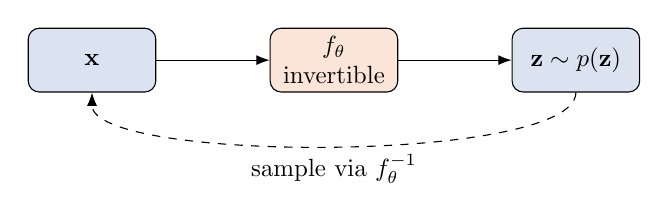
\begin{tikzpicture}[node distance=1.1cm]
    \tikzstyle{box}=[draw, rounded corners, minimum width=1.8cm, minimum height=0.9cm, align=center]
    \node[box, fill=myblue!15] (x) {$\mathbf{x}$};
    \node[box, right=1.6cm of x, fill=myorange!15] (f) {$f_\theta$\\invertible};
    \node[box, right=1.6cm of f, fill=myblue!15] (z) {$\mathbf{z}\sim p(\mathbf{z})$};
    \draw[-{Latex}] (x) -- (f);
    \draw[-{Latex}] (f) -- (z);
    \draw[-{Latex}, dashed] (z.south) .. controls +(0,-1.0) and +(0,-1.0) .. (x.south)
      node[midway, below] {sample via $f_\theta^{-1}$};
  \end{tikzpicture}
\end{adjustbox}

\vspace{0.55em}
\textbf{Log-likelihood}
\[
  \log p_\theta(\mathbf{x})=\log p(\mathbf{z})+
  \log\left|\det \frac{\partial f_\theta(\mathbf{x})}{\partial \mathbf{x}}\right|,\quad
  \mathbf{z}=f_\theta(\mathbf{x}).
\]
\textbf{Notes:} RealNVP/Glow (coupling), spline flows, CNFs/Neural ODEs.
\end{frame}

% ================= Section ==================
\section{Diffusion / Score-based Models}

\begin{frame}{Diffusion models: Forward and Reverse Processes}
\centering
\begin{adjustbox}{max size={\linewidth}{.50\textheight}}
  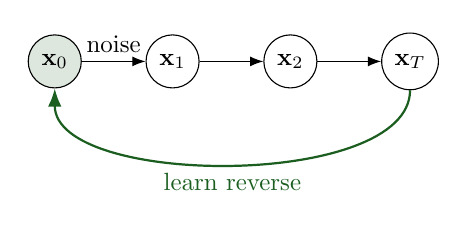
\begin{tikzpicture}[node distance=0.9cm]
    \tikzstyle{round}=[draw, circle, minimum size=7mm]
    \node[round, fill=mygreen!15] (x0) {$\mathbf{x}_0$};
    \node[round, right=0.9cm of x0] (x1) {$\mathbf{x}_1$};
    \node[round, right=0.9cm of x1] (x2) {$\mathbf{x}_2$};
    \node[round, right=0.9cm of x2] (xT) {$\mathbf{x}_T$};
    \draw[-{Latex}] (x0) -- (x1) node[midway, above] {noise};
    \draw[-{Latex}] (x1) -- (x2);
    \draw[-{Latex}] (x2) -- (xT);
    \draw[-{Latex}, thick, mygreen] (xT.south) .. controls +(0,-1.4) and +(0,-1.4) .. (x0.south)
      node[midway, below] {learn reverse};
  \end{tikzpicture}
\end{adjustbox}

\vspace{0.4em}
\small
\textbf{Parameterizations \& losses}
\begin{itemize}
  \item \textbf{Noise ($\varepsilon$)-prediction}:
  \[
    \mathcal{L}_\varepsilon
     = \mathbb{E}_{\mathbf{x}_0,t,\varepsilon}\!\left[
       w_t\,\|\varepsilon-\varepsilon_\theta(\mathbf{x}_t,t)\|^2\right],\quad
     \mathbf{x}_t=\sqrt{\bar\alpha_t}\,\mathbf{x}_0+\sqrt{1-\bar\alpha_t}\,\varepsilon.
  \]
  \item \textbf{$x_0$-prediction}:
  \[
    \mathcal{L}_{x_0}
     = \mathbb{E}_{\mathbf{x}_0,t,\varepsilon}\!\left[
       w_t\,\|\mathbf{x}_0-\hat{\mathbf{x}}_{0,\theta}(\mathbf{x}_t,t)\|^2\right],\quad
     \varepsilon_\theta=\frac{\mathbf{x}_t-\sqrt{\bar\alpha_t}\,\hat{\mathbf{x}}_{0,\theta}}{\sqrt{1-\bar\alpha_t}}.
  \]
  \item \textbf{Score model (DSM)}:
  \[
    \mathcal{L}_\text{DSM}
      = \mathbb{E}_{t,\mathbf{x}_0}\,
        \mathbb{E}_{\mathbf{x}_t\sim q(\cdot\mid\mathbf{x}_0)}
        \!\left[\lambda(t)\,\|s_\theta(\mathbf{x}_t,t)-\nabla_{\mathbf{x}_t}\log q(\mathbf{x}_t\mid\mathbf{x}_0)\|^2\right].
  \]
\end{itemize}
\end{frame}

\begin{frame}{Flow Matching}
  \small
  Train a velocity field $\mathbf{v}_\theta(\mathbf{x},t)$ moving $p_0\to p_1$ by the ODE
  \[
    \frac{d\mathbf{x}}{dt}=\mathbf{v}_\theta(\mathbf{x},t),\quad
    \mathbf{x}(0)\sim p_0,\ \mathbf{x}(1)\sim p_1\approx p_{\text{data}}.
  \]
  
  \textbf{Loss (conditional flow matching)}
  \[
    \mathcal{L}_{\mathrm{CFM}}
    = \mathbb{E}_{t\sim\mathcal{U}(0,1)}
      \ \mathbb{E}_{\mathbf{x}_0\sim p_0,\ \mathbf{x}_1\sim p_1}
      \ \mathbb{E}_{\mathbf{x}_t=(1-t)\mathbf{x}_0+t\mathbf{x}_1}
      \Big[\ \|\mathbf{v}_\theta(\mathbf{x}_t,t)-(\mathbf{x}_1-\mathbf{x}_0)\|^2\ \Big].
  \]
  \textit{General path form} (with path density $\pi_t$ and target drift $\mathbf{u}_t$):
  \[
    \mathcal{L}
    = \mathbb{E}_{t,\mathbf{x}_0,\mathbf{x}_1,\mathbf{x}_t\sim \pi_t(\cdot|\mathbf{x}_0,\mathbf{x}_1)}
      \Big[\ \|\mathbf{v}_\theta(\mathbf{x}_t,t)-\mathbf{u}_t(\mathbf{x}_0,\mathbf{x}_1,t)\|^2\ \Big].
  \]
  
  \textbf{Perks:} simple targets; few-step sampling; latent-friendly.
  \end{frame}

% ================= Section ==================
\section{Modern Hybrids and Trends}

\begin{frame}{Converging Lines}
\begin{itemize}
  \item \textbf{Tokenizer + AR + Diffusion:} VQ-VAE/LDM token spaces with AR planning/control.
  \item \textbf{Flow Matching \/ Rectified Flow:} train a velocity field $\mathbf{v}_\theta(\mathbf{x},t)$ to move noise$\to$data with 1st-order ODE sampling.
  \item \textbf{Consistency Models:} distilled one-step or few-step samplers by self-consistency constraints.
  \item \textbf{Mean Flow:} train an averaged velocity for one step generation.
  \item \textbf{Multimodal, Video, 3D/4D:} text-image-audio-video-geometry; world-model style conditional generation.
\end{itemize}
\vspace{0.3em}
\textbf{Takeaway:} boundaries blur; choose representations (continuous vs. discrete tokens), objectives, and samplers to fit task/latency.
\end{frame}

% ================= Section ==================
\section{Evaluation: Metrics and Pitfalls}

\begin{frame}{How We Measure}
\begin{itemize}
  \item \textbf{Likelihood / BPD}: exact (AR/flows) or bounds (VAE); diffusion often uses NLL surrogates.
  \item \textbf{Sample Quality}: FID, KID, IS; CLIP-score for text-image alignment.
  \item \textbf{Diversity/Coverage}: precision\&recall for distributions; recall of rare modes.
  \item \textbf{Task Utility}: downstream performance, human eval.
\end{itemize}
\end{frame}

% ================= Section ==================
\section{Choosing the Right Family}

% ---- Decision Guide inserted ----
\begin{frame}{Decision Guide: Which Family Should I Choose?}
\small
\begin{itemize}
  \item \textbf{Need exact likelihood / lossless compression?} $\,\Rightarrow\,$ Autoregressive or Flows.
  \item \textbf{Top visual fidelity / editing?} $\,\Rightarrow\,$ Diffusion (latent), consider consistency/rectified/flow matching for speed.
  \item \textbf{Discrete tokens (text/code) or controllable sequences?} $\,\Rightarrow\,$ Autoregressive (Transformer) \,+ tokenizers for images/audio.
  \item \textbf{Low-latency sampling at inference?} $\,\Rightarrow\,$ GANs/consistency/flow-matched diffusion; Flows when feasible.
  \item \textbf{Structured latent space / downstream control?} $\,\Rightarrow\,$ VAE/Hierarchical VAE (+ AR or diffusion decoders).
\end{itemize}
\end{frame}

\begin{frame}{Practical Trade-offs}
\small
\begin{table}
\centering
\begin{tabular}{@{}lccccc@{}}
\toprule
\textbf{Family} & \textbf{Likelihood} & \textbf{Quality} & \textbf{Speed (sample)} & \textbf{Control} & \textbf{Stability}\\
\midrule
Autoregressive & \cmark & \cmark (text/code) & \xmark & \cmark & \cmark\\
VAE & bound & mixed & \cmark & \cmark & \cmark \\
GAN & \xmark & \cmark & \cmark & mixed & mixed \\
NFlows & \cmark & mixed & mixed & \cmark & \cmark\\
Diffusion & bound & \cmark & mixed$\to$\cmark & \cmark & \cmark\\
\bottomrule
\end{tabular}
\end{table}
\vspace{2em}
\textbf{Takeaway:} Disrete, latent space, mode collapse, inverse design with exact log likelihood, high quality samples with few-steps.
\end{frame}

% ================= Section ==================
\section{Case Studies / Applications}

\begin{frame}{Applications (Examples)}
\begin{itemize}
  \item \textbf{Images/Design}: product ideation, content creation, inpainting/outpainting.
  \item \textbf{Text/Code}: LLMs for writing, agents, program synthesis.
  \item \textbf{Audio/Speech/Music}: TTS, music generation, audio restoration.
  \item \textbf{Video/World Models}: controllable video, simulation for planning.
  \item \textbf{3D/Geometry}: NeRF/mesh diffusion, 3D asset pipelines.
  \item \textbf{Science}: molecules/proteins/materials; weather/climate surrogates.
\end{itemize}
\end{frame}

\begin{frame}
\begin{figure}
\centering
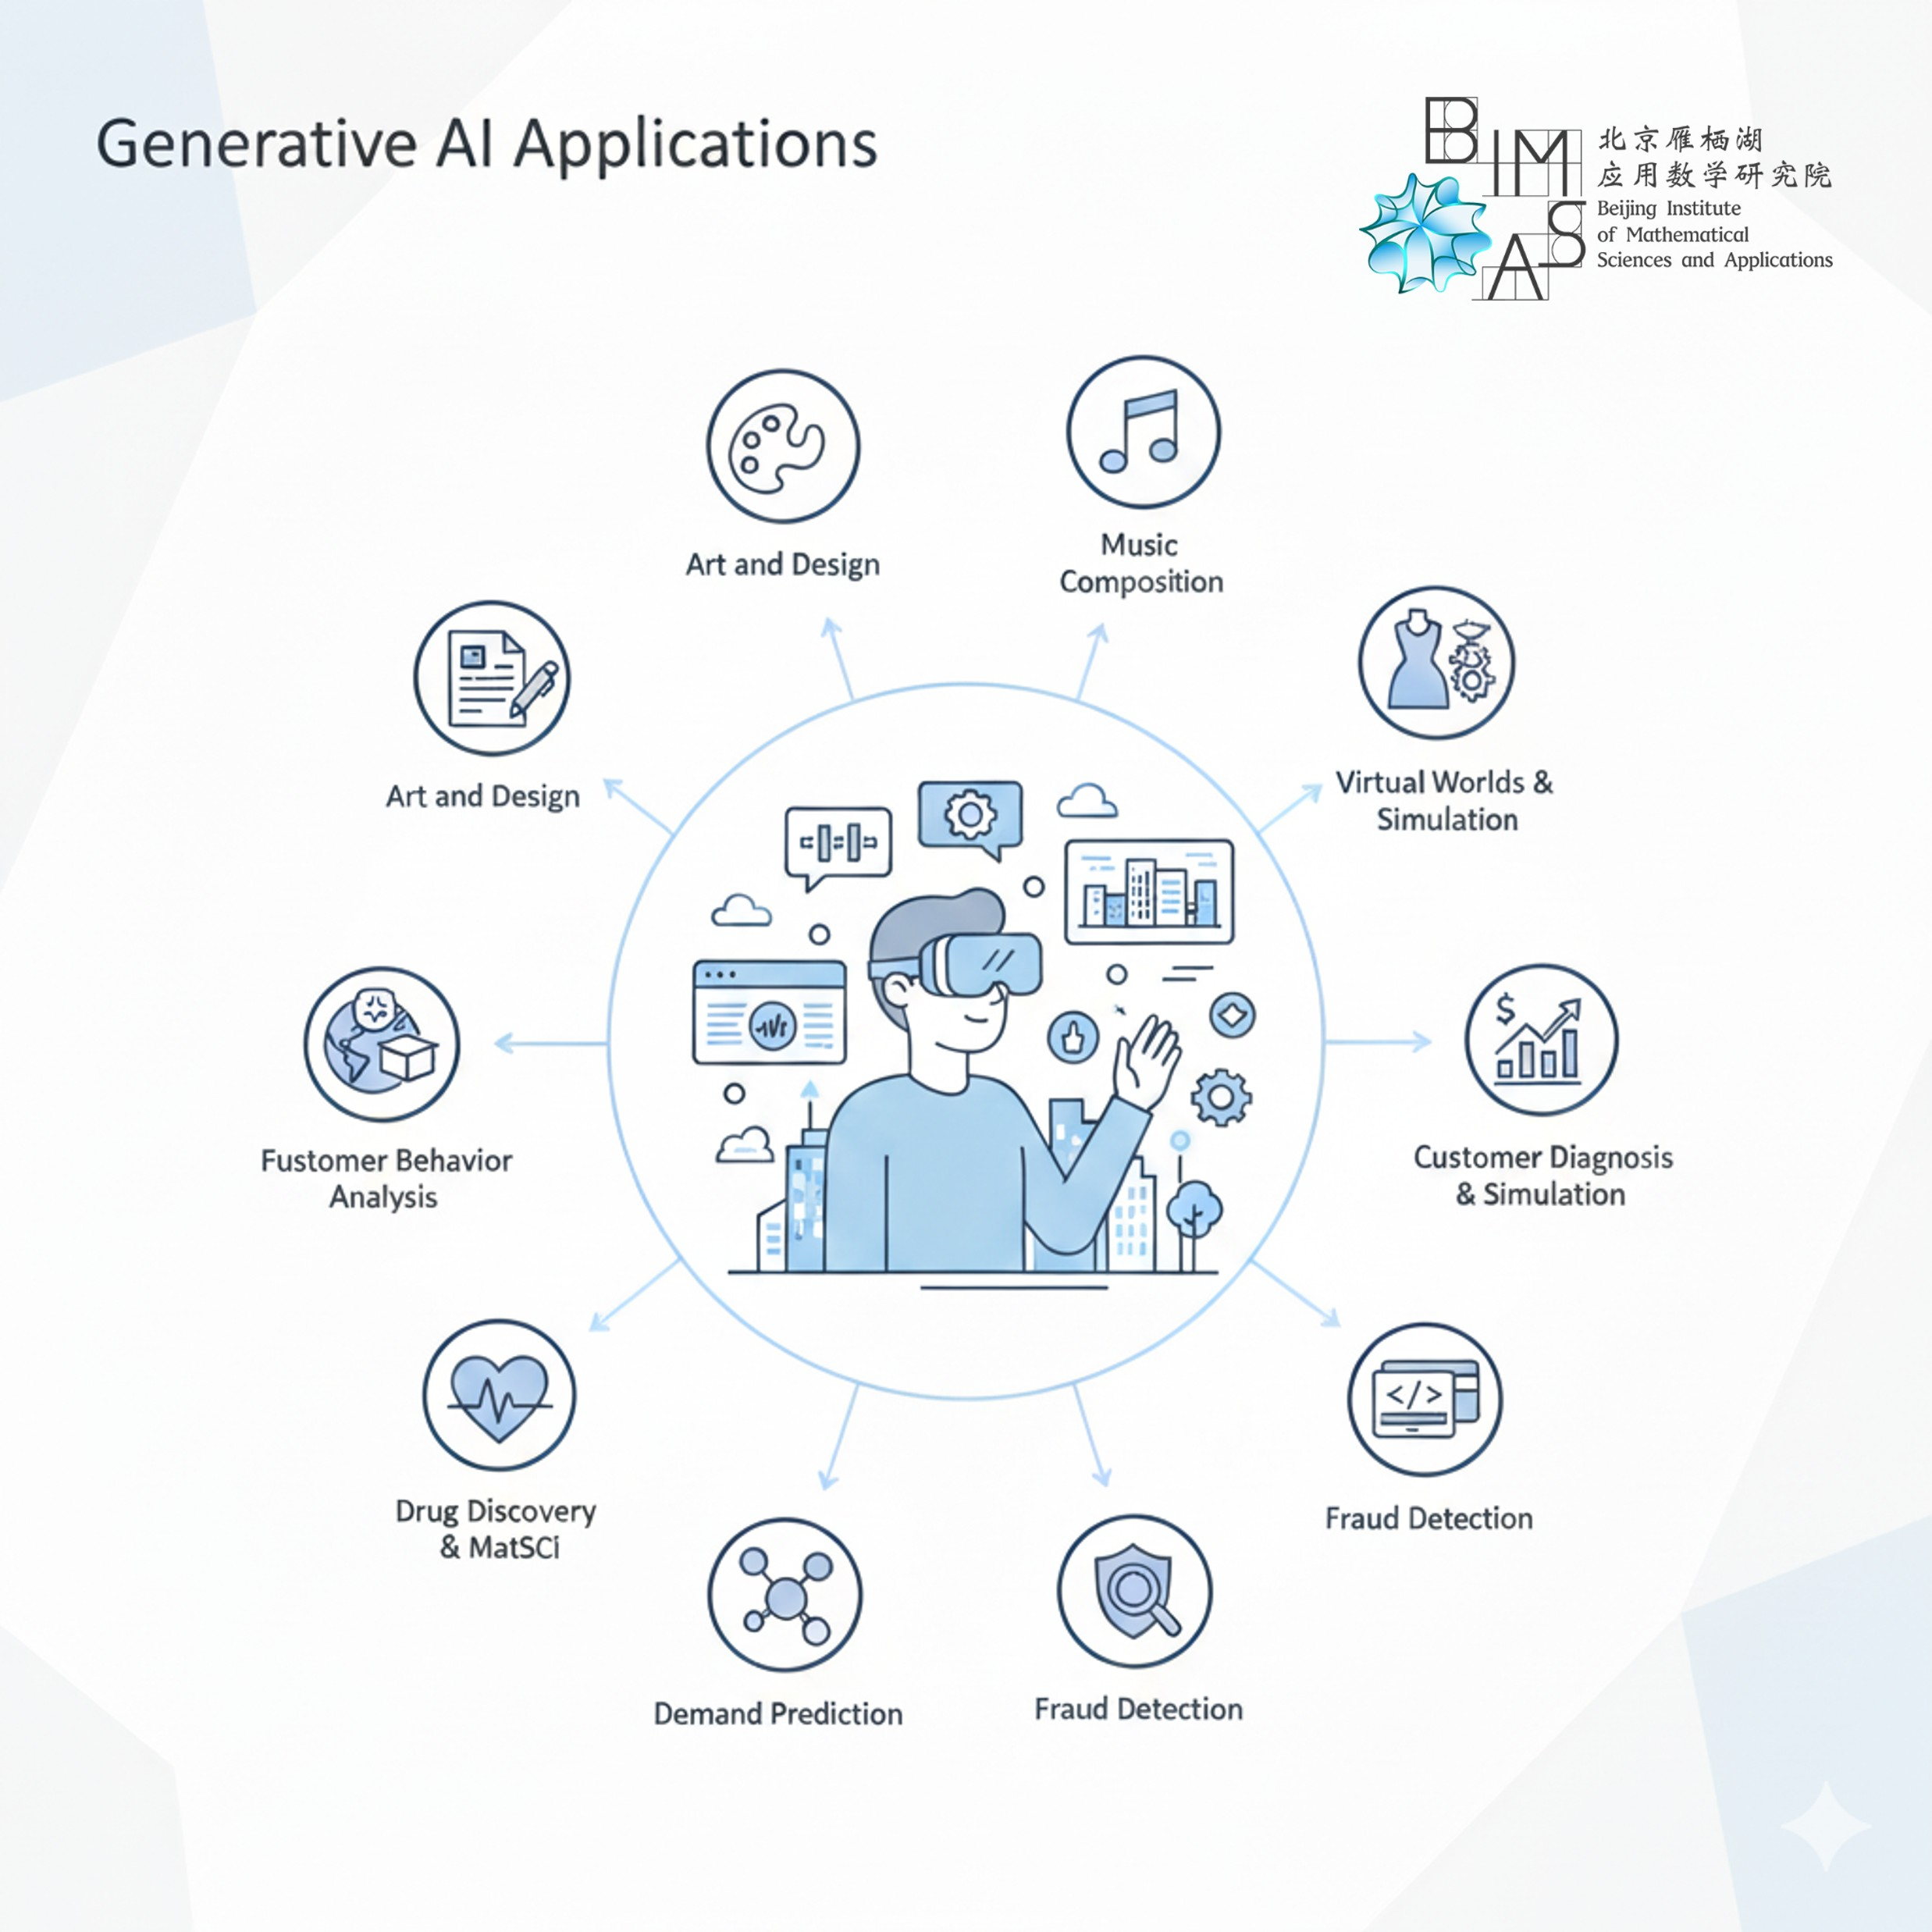
\includegraphics[width=0.5\textwidth]{figs/generative_ai.jpg}
\end{figure}
\end{frame}

% ================= Section ==================
\section{World Models}

% ---- Positioning slide ----
\begin{frame}{Positioning: From Generative Models to World Models}
\small
\begin{itemize}
  \item \textbf{Observation model:} generative $p(\mathbf{o}_t \mid \mathbf{z}_t)$ often shares tech with diffusion/AR/VAEs.
  \item \textbf{Dynamics:} latent transition $f_\theta(\mathbf{z}_{t+1}\mid\mathbf{z}_t, \mathbf{a}_t)$ (Dreamer/JEPA-style) or direct video simulators.
  \item \textbf{Control:} plan over imagined rollouts (MPC) or learn policy $\pi(\mathbf{a}_t\mid\mathbf{z}_t)$.
  \item \textbf{Bridges:} AR for tokens (language/code); diffusion for frames; flows/consistency/flow-matching for speed.
\end{itemize}
\end{frame}

\begin{frame}{World Models: A Compact Overview (2025)}
\vspace{0.5em}
\begin{itemize}
  \item \textbf{Goal:} learn $p(\mathbf{o}_{t+1}\mid\mathbf{o}_t,\mathbf{a}_t)$ or latent dynamics $f_\theta$; plan via MPC or policy over imagined trajectories.
  \item \textbf{Two flavors:} (i) action-conditioned \emph{video/world simulators}; (ii) representation-first models (e.g., latent JEPA/Dreamer-style) for control/planning.
  \item \textbf{Training signals:} next-frame/latent prediction, contrastive/self-supervision, auxiliary reward/value heads.
  \item \textbf{Eval:} physical plausibility, action-consistency, controllability, and task success; long-horizon memory.
  \item \textbf{Open issues:} causality/counterfactuals, persistent memory/state, sim-to-real, safety.
\end{itemize}
\end{frame}

\begin{frame}
  \centering
\begin{adjustbox}{max size={\linewidth}{.50\textheight}}
  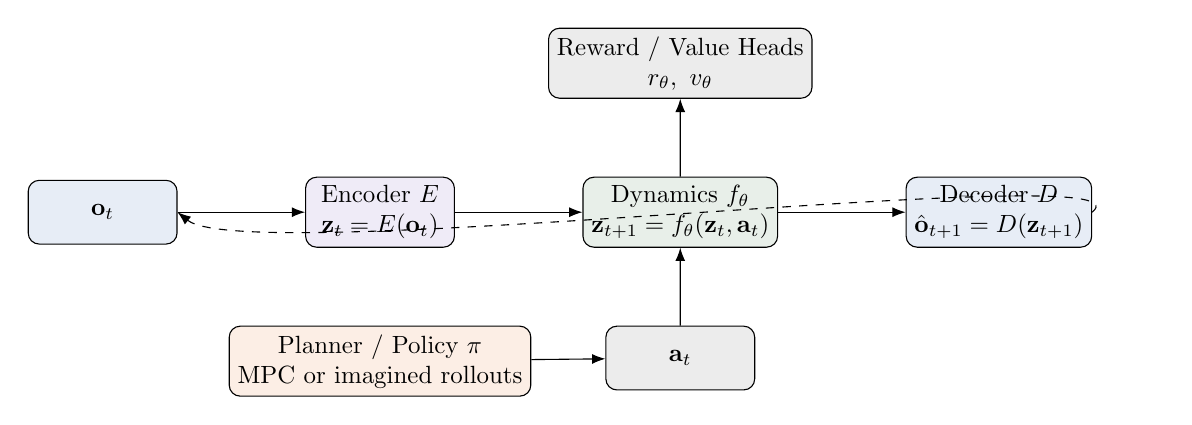
\begin{tikzpicture}[node distance=1.4cm]
    \tikzstyle{box}=[draw, rounded corners, minimum width=2.1cm, minimum height=0.9cm, align=center]
    % Observations and actions
    \node[box, fill=myblue!10] (ot) {$\mathbf{o}_t$};
    \node[box, right=1.8cm of ot, fill=myviolet!10] (enc) {Encoder $E$\\$\mathbf{z}_t=E(\mathbf{o}_t)$};
    \node[box, right=1.8cm of enc, fill=mygreen!10] (dyn) {Dynamics $f_\theta$\\$\mathbf{z}_{t+1}=f_\theta(\mathbf{z}_t,\mathbf{a}_t)$};
    \node[box, right=1.8cm of dyn, fill=myblue!10] (dec) {Decoder $D$\\$\hat{\mathbf{o}}_{t+1}=D(\mathbf{z}_{t+1})$};
    \draw[-{Latex}] (ot) -- (enc);
    \draw[-{Latex}] (enc) -- (dyn);
    \draw[-{Latex}] (dyn) -- (dec);
    % Planner / action
    \node[box, below=1.1cm of enc, fill=myorange!10] (pi) {Planner / Policy $\pi$\\MPC or imagined rollouts};
    \node[box, below=1.1cm of dyn, fill=gray!15] (a) {$\mathbf{a}_t$};
    \draw[-{Latex}] (pi) -- (a);
    \draw[-{Latex}] (a) -- (dyn);
    % Value / reward heads
    \node[box, above=1.1cm of dyn, fill=gray!15] (val) {Reward / Value Heads\\$r_\theta,\ v_\theta$};
    \draw[-{Latex}] (dyn) -- (val);
    % Feedback
    \draw[-{Latex}, dashed] (dec.east) .. controls +(1.0,0.8) and +(1.0,-0.8) .. (ot.east);
  \end{tikzpicture}
\end{adjustbox}
\\
\vspace{2em}
\textbf{Takeaway:} World Models are systems that learn the dynamics of an environment to plan and control actions by imagining future outcomes, but still face key challenges in causality, memory, and real-world application. 
\end{frame}

% ================= Section ==================
\section{Summary}

\begin{frame}{Key Messages}
\begin{enumerate}
  \item \textbf{Five pillars:} AR, VAE, GAN, Flows, Diffusion. Each optimizes a different compromise.
  \item \textbf{Autoregression} remains the gold standard for discrete sequences; for continuous media, tokenization + AR is powerful.
  \item \textbf{Diffusion/Score-based} dominates visual fidelity; distillation and flow-matching narrow the latency gap.
  \item \textbf{Hybrids} are the 2025 norm: choose representation + objective + sampler for your latency/quality/control budget.
\end{enumerate}
\end{frame}

% ================= Section ==================
\section*{Further Reading}

\begin{frame}{Pointers (non-exhaustive)}
\small
\begin{itemize}
  \item \textbf{AR:} PixelRNN/CNN; GPT-style Transformers for text/code; VQ-VAE + Transformer for images/audio.
  \item \textbf{VAE:} Kingma and Welling (2014); Hierarchical/$\beta$-VAE; VQ-VAE.
  \item \textbf{GAN:} Goodfellow et al. (2014); WGAN, StyleGAN series.
  \item \textbf{Flows:} RealNVP, Glow; Neural ODEs; spline flows.
  \item \textbf{Diffusion/Score:} Sohl-Dickstein (2015), DDPM, DDIM, LDM; consistency/rectified/flow-matching; DPM-Solver.
\end{itemize}
\end{frame}

\end{document}
